\documentclass[12pt]{article}

\usepackage[italicdiff]{physics}
\usepackage[margin=0.6in]{geometry}
\usepackage{amsmath}
\usepackage{bm}
\usepackage{hyperref}
\usepackage{graphicx}
\usepackage{amssymb}
\usepackage{bbm}

\numberwithin{equation}{section}

\title{Homework \#10 \\ MA391}
\author{Will Bodron}

\setcounter{section}{17}

\begin{document}
    \section{Problem}
    \paragraph{} Consider a $5\times5$ grid. We say a \textit{valid} districting plan is one that uses five contiguous districts with five squares each. Let us call a district a \textit{line} if it is five squares in a row.
    \begin{enumerate}
        \item Show that there are two valid plans that use five lines in a $5\times5$ grid.
        \paragraph{} Choose draw a line district anywhere. There are 10 ways to do this. 5 of these ways result in plans that are completely made of vertical lines, and the other 5 ways result in plans that are made up of horizontal lines.

        
\includegraphics[width=0.3\textwidth]{figures/vstripes.png}
        
\includegraphics[width=0.3\textwidth]{figures/vstripes.png}
        \item Explain why there are the same number of valid plans using at least four lines as using exactly five lines.
        \paragraph{} A complete plan contains 5 districts. If we have four lines in a plan, the 5th district must be composed entirely of the remaining 5 squares $(25-4*5) = 5$. There is only one way to make a 5th district out of 5 squares, so every plan with at least 4 lines is the same as one plan with 5 lines (and vice versa). Since there is a isomorphism between the groups, they must have the same size.
        \item Let $M$ be the number of valid districting plans for a $2\times5$ grid, using two contiguous districts with five squares each, where none of the districts are lines. Find $M$ and prove your answer is correct.
        \paragraph{} Inspired by the MCMC sampling method of transforming a districting plan into a new one, we'll do the same to find the number of plans here. For the case of two lines on a $2\times5$ grid, there are only two flip moves that result in a valid district. These are swapping two opposite corners.
        
\includegraphics[width=0.3\textwidth]{figures/plan_0.png}
        
\includegraphics[width=0.3\textwidth]{figures/plan_1.png}
        \paragraph{} After doing this action, we realize it might've been nicer to pick a transformation that could be repeated. In fact there is such a transformation, whose repeated application that cycles through all districts. You're probably familiar with it if you've played the retro arcade game Snake. Taking one side of the line to be the head, move the snake through the grid, moving `forward' and avoiding walls and your tail.

        
\includegraphics[width=0.25\textwidth]{figures/plan_2.png}
        
\includegraphics[width=0.25\textwidth]{figures/plan_3.png}
        
\includegraphics[width=0.25\textwidth]{figures/plan_4.png}
        \paragraph{} After one final application of the transformation, we will have returned to where we came, except the colors have switched. This must be all the plans, because we've come full circle, and there was only one possible move (that didn't return us to one that we've already seen) at every stage. Remove the plan that was two lines, as prescribed by the prompt, and $M=4$ valid plans remain.
        
        \item Prove that the number of valid plans for a $5\times5$ grid using exactly three lines is 8M.
        There are 4 ways to leave 2 adjacent rows unfilled by horizontal districts, (and ditto vertically). The 2 adjacent columns (or rows) can be filled with $M$ districts, since it must be cover a $2\times5$ grid.
        $$4\times2\times M$$
    \end{enumerate}
    \section{Problem}
    In an $8\times8$ grid, place 43 ``blue'' voters and 21 ``red'' votes and assign them to four districts satisfying the following conditions:
    \begin{enumerate}
        \item Each district is connected/contiguous
        \item Each district has at least 12 squares
        \item Three districts contain a majority of red voters and one district contains a majority of blue voters.
    \end{enumerate}
    Create a 2d plot containing four points where the $x$-values correspond to the percentage of ``red'' voters in district $x$

    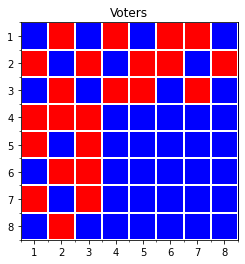
\includegraphics[width=0.45\textwidth]{figures/voters.png}
    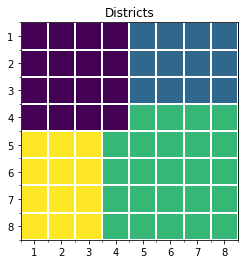
\includegraphics[width=0.45\textwidth]{figures/districts.png}
    
    This problem can be dealt with by putting the blue voters packed in a large district. Clearly district 2 is the largest, green district.
    
    \begin{center}
        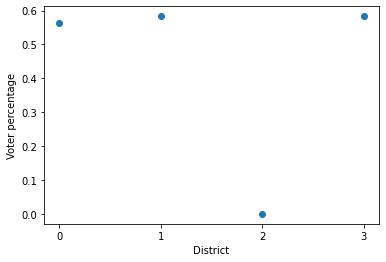
\includegraphics[width=0.75\textwidth]{figures/percentage.png}
    \end{center}

    \section{Problem}
    Similar to problem 19, in an $8\times8$ grid, place 43 ``blue'' voters and 21 ``red'' votes and assign them to four districts satisfying the following conditions:
    \begin{enumerate}
        \item Each district is connected/contiguous
        \item Each district has at least 12 squares
        \item All four districts contain a majority of blue voters
        \item All four districts have a different number of blue voters
    \end{enumerate}
    Create a 2d plot containing four points where the $x$-values correspond to the percentage of ``red'' voters in district $x$.

    These conditions are relatively probable for a randomly generated set of 43 and 21 voters on equally sized districts. After finding a voter configuration that satisfied the first 3 conditions, I changed it manually to make all the districts have a different number of blue voters.

    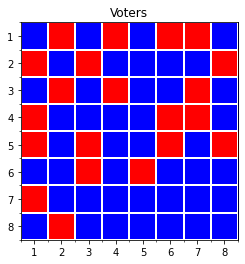
\includegraphics[width=0.45\textwidth]{figures/voters20.png}
    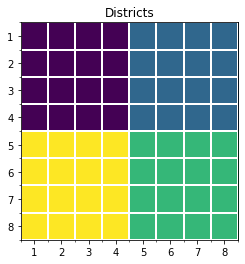
\includegraphics[width=0.45\textwidth]{figures/districts20.png}

    \begin{center}
        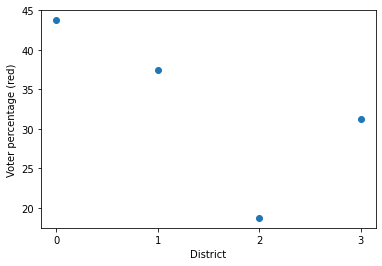
\includegraphics[width=0.75\textwidth]{figures/percentage20.png}
    \end{center}

    \setcounter{section}{7}
    \section{Essay}
    \paragraph{} Throughout my math education I have sensed a disconnect between what and how I'm learning and how math is performed professionally. I think this presents itself especially in the majority of homeworks I have done up until my senior year. Traditionally, a problem set is prompting students to replicate something already seen or apply something slightly differently. The assignment to investigate the Riemann hypothesis was something completely different from this norm. I'd never spend time to be really exploratory and creative within the context of a complicated problem. Carry out to dead ends and learn something. In other contexts (quantum mechanics), because of the sheer size of our problem sets, any sort of thought spent on a `dead ends' is just a waste of time I could've copying proofs from our textbook.
    \paragraph{} Introspectively, I'm drawn to this sort of exercise I'm especially motivated by novelty. At any and all chances, I'll take the creative route. Even on this assignment 10 about gerrymandering, I saw the prompts and knew I should start building a quicker system for visualizing districts and voters. Certainly there are easier ways to draw squares, and the final execution could've used some improvement. I'll excuse the execution because I'm on a time crunch and telling myself that this small creative pursuit shouldn't get in the way of returning an assignment on time. I do, however, feel I've benefitted from this exercise of writing code to generate images. Outside of the clear lessons about district shape and voters, I've created (or started the process) of my own work within the field. Additionally, these lessons in 2d image creation from data can no doubt be used in all kinds of contexts.
    \paragraph{} I think I've always known that I'm motivated by creativity, and used it to my advantage at times. At times I'll convince myself to work on something I'm reluctant or uninterested in by transforming, at least very slightly, the process of that creation into something that I can find incredibly creatively stimulating.
    \paragraph{} On the same coin, assignments where I struggle to find creative leeway are far more difficult for me. Assignment 3 and 6 are representations of this for me. In no way am I saying these are bad assignments, but they do feel more `scripted' than others. Now perhaps I just wasn't creative enough to come up with extraneous solutions to the problems given, but I think we can all agree that explaining someone else's proof or following the hints is slightly less rewarding than going off on your own to find something. There however is clearly an advantage to following a list of questions. These are the questions (or similar ones) that led original mathematicians to very large claims. Posing numerous and valuable questions is what sets the best mathematicians apart from those learning to be the best. Problems 14 and 15,
    proving the claims about primes through a conversation about square-free numbers was particularly difficult. My answer represents every quantity as a product using the grotesque $\prod$ notation. It feels very much like I've translated the question and gotten to an answer without any work, indicating, that perhaps all the work of proving claims about primes was done in the wording of these questions. Perhaps the frustration that I've felt with this is that I would certainly struggle significantly to come up with questions about square-freeness in the context of primes, and even if I did, I may not have recognized its values. I'm given rest again once I remember that these topics we've done in class in a week or two were done originally by mathematicians over centuries.

\end{document}